\documentclass[a4paper,12pt]{article} 


\usepackage[T2A]{fontenc}			
\usepackage[utf8]{inputenc}			
\usepackage[english,russian]{babel}	

\usepackage{graphicx, scalerel}    
\usepackage{wrapfig}               
\usepackage[14pt]{extsizes}        
\usepackage[warn]{mathtext}       
\usepackage{indentfirst}      
\usepackage[margin = 25mm]{geometry}
\usepackage[table,xcdraw]{xcolor} 
\usepackage{amsmath,amsfonts,amssymb,amsthm,mathtools}
\usepackage{wasysym}                
\usepackage{upgreek}                
\usepackage{caption}
\usepackage{multirow}
\captionsetup{labelsep=period}
\usepackage[font=small,labelfont=bf]{caption}
\usepackage{gensymb}
\usepackage[unicode, pdftex]{hyperref}
\usepackage{tikz}
\usetikzlibrary{positioning}
\usepackage{fancyhdr}
\pagestyle{fancy}
\setlength\fboxsep{3pt} % Отступ рамки \fbox{} от рисунка
\setlength\fboxrule{1pt} % Толщина линий рамки \fbox{}
\newcommand{\tocsection}[1]{\section*{#1} \addcontentsline{toc}{section}{#1}}
\newcommand{\tocsubsection}[1]{\subsection*{#1} \addcontentsline{toc}{subsection}{#1}}
\renewcommand{\cftsecleader}{\cftdotfill{\cftdotsep}}

\def\fillandplacepagenumber{%
	\par\pagestyle{empty}%
	\vbox to 0pt{\vss}\vfill
	\vbox to 0pt{\baselineskip0pt
		\hbox to\linewidth{\hss}%
		\baselineskip\footskip
		\hbox to\linewidth{%
			\hfil\thepage\hfil}\vss}}

\begin{document}
		\newcommand{\HRule}{\rule{\linewidth}{0.7mm}} % Defines a new command for the horizontal lines, change thickness here

\begin{center}
	\large\textbf{Московский Физико-Технический Институт}\\
	\large\textbf{(государственный университет)}
	
	\vfill
	

	
	\Large Вычислительная математика
	%----------------------------------------------------------------------------------------
	%	TITLE SECTION
	%----------------------------------------------------------------------------------------
	
	\HRule
	\\[0.4cm]
	{ \huge \bfseries Лабораторная работа №9}
	\\[0.4cm] % Title of your document
	\HRule
	\\[0.5cm]
	
	\ \\
	\textbf{\large Автор:} \\	
	\large Овсянников Михаил Б01-008\\
	\vfill
	\hspace*{-0.8 cm}
\includegraphics[width=100 pt]{./Include/frkt_logo.pdf}\\
	\large Долгопрудный, 2023
\end{center}

\thispagestyle{empty}

\newpage
\setcounter{page}{2}
\fancyfoot[c]{\thepage}
\fancyhead[L] {Лабораторная работа №9}
\fancyhead[R]{}

		\tableofcontents
		\newpage
		
		\tocsection{Цель}
		Реализовать методы решения жестких систем ОДУ.
			
		\tocsection{Теоретические сведения}
		\tocsubsection{Общая задача}

		Пусть у нас есть система ОДУ:
		\begin{equation*}
			\begin{cases}
				y'(x) = f(x, y),\\
				y(x_0) = y_0.
			\end{cases}
		\end{equation*}
		
		Требуется численно решить данную систему. Для этого есть множество методов, однако некоторые из них могут оказаться неустойчивыми для данной системы и решение будет посчитано неверно, уйдет в бесконечность или начнет сильно осциллировать. Это происходит потому, что система может оказаться жесткой, то есть спектр матрицы Якоби данной системы распадается на две части:
		\begin{itemize}
			\item Жесткая
			\begin{flalign*} 
				&\text{Re}{\lambda_i} \leqslant -\Lambda_0, \text{ где } \Lambda_0 > 0,& \\
				&|\text{Im}\lambda_i| < |\text{Re}\lambda_i|, \;\;\;\;\;\;\; i = 1, 2, ..., N_1;&
			\end{flalign*}
		
			\item Нежесткая
			\begin{flalign*} 
				&|\lambda_i| \leqslant \lambda_0,  \;\;\;\;\;\;\;\;\;\;\;\;\;\;\;\;\; i = N_1 + 1, ..., N;&
			\end{flalign*}
		\end{itemize}
		И $q = \Lambda_0/\lambda_0 \gg 1$ -- число жесткости.
		
		На практике легко определить жесткую систему, когда её собственные значения сильно расходятся по порядку.
		
		Выход из столь неприятной ситуации -- использовать устойчивые методы. Например, такие как неявные методы Рунге-Кутты, многостадийные методы Розенброка или неявные многошаговые методы. В данной работе как раз реализован трехстадийный метод Розенброка для решения жесткой системы обыкновенных дифференциальных уравнений.
		
		
		\newpage
		\tocsubsection{Описание трехстадийного метода Розенброка}
		Все методы Розенброка основаны на том, что мы линеаризируем правую часть уравнения и на каждом шаге решаем СЛАУ. Конкретно для трехстадийного процедура выглядит так:
		\begin{equation*}
			y_{n+1} = y_n + p_1 k_1 + p_2 k_2 + p_3 k_3,
		\end{equation*}
	
		\noindent где:
		\begin{equation*}
			\begin{split}
				D_n k_1 &= hf(x_n, y_n), \\
				D_n k_2 &= hf(x_n + \beta_{21}h, y_n + \beta_{21} k_1), \\
				D_n k_3 &= hf(x_n + (\beta_{31} + \beta_{32})h, y_n + \beta_{31} k_1 + \beta_{32} k_2)),\\
				\\
				D_n \;\; &= E - ah\frac{\partial f}{\partial y}(x_n, y_n).
			\end{split}
		\end{equation*}
		
		Здесь $a, p_i, \beta_{ij}$ -- действительные числа. Конкретно:
		\begin{equation*}
			\begin{split}
				a   &= \;\;\, 0.435866521508 \\
				p_1 &= \;\;\, 0.435866521508 \\
				p_2 &= \;\;\, 0.478240833275 \\
				p_3 &= \;\;\, 0.085892645217 \\
				\beta_{21} &= \;\;\, 0.435866521508 \\
				\beta_{31} &= \;\;\, 0.435866521508 \\
				\beta_{32} &= -2.116053335950
			\end{split}
		\end{equation*}
	
		То есть на каждом шаге интегрирования нам нужно решить 3 СЛАУ.
		
		\tocsection{Сама система}
		\tocsubsection{Постановка задачи}
		В качестве примера жесткой системы ОДУ был выбран номер \textbf{X.9.8} второй части сборника Аристовой и Лобанова:
		\begin{equation*}
			\begin{cases*}
				\dot{x} = 77.27(y + x (1 - 8.375 \cdot 10^{-6} x - y)), \\
				\dot{y} = \frac{1}{77.27}(z - (1 + x)y), \\
				\dot{z} = 0.161(x - z).
			\end{cases*}
		\end{equation*}
	
		В качестве начального значения выбран вектор $(x \;\; y \;\; z)^T_0 = (4 \;\; 1.1 \;\; 4)^T$.
		
		Данная система является математической моделью Филда–Нойса <<орегонатор>> периодической химической реакции		Белоусова–Жаботинского.
		
		Видно, что данная система является жесткой, так как есть сильные различия в <<константах скорости реакций>> веществ X, Y и Z.
		
		На каждом шаге интегрирования мы будем решать 3 системы линейных алгебраических уравнений. Для этого будем использовать метод верхней релаксации.
		
		\tocsubsection{Результаты}
		Процесс решения достаточно долгий ввиду того, что нужно решать еще 3 СЛАУ на каждом шаге интегрирования. На машине с процессором AMD Ryzen 5 3500U with Radeon Vega Mobile Gfx 2.10 GHz расчет по имеющемуся коду занял 112 секунд для 80000 итераций с шагом интегрирования $h = 10^{-2}$.
		
		Однако результат того стоит. Система была спокойно решена. Предоставим зависимость $x, y$ и $z$ от времени:
		\begin{figure}[h!]
			\centering
			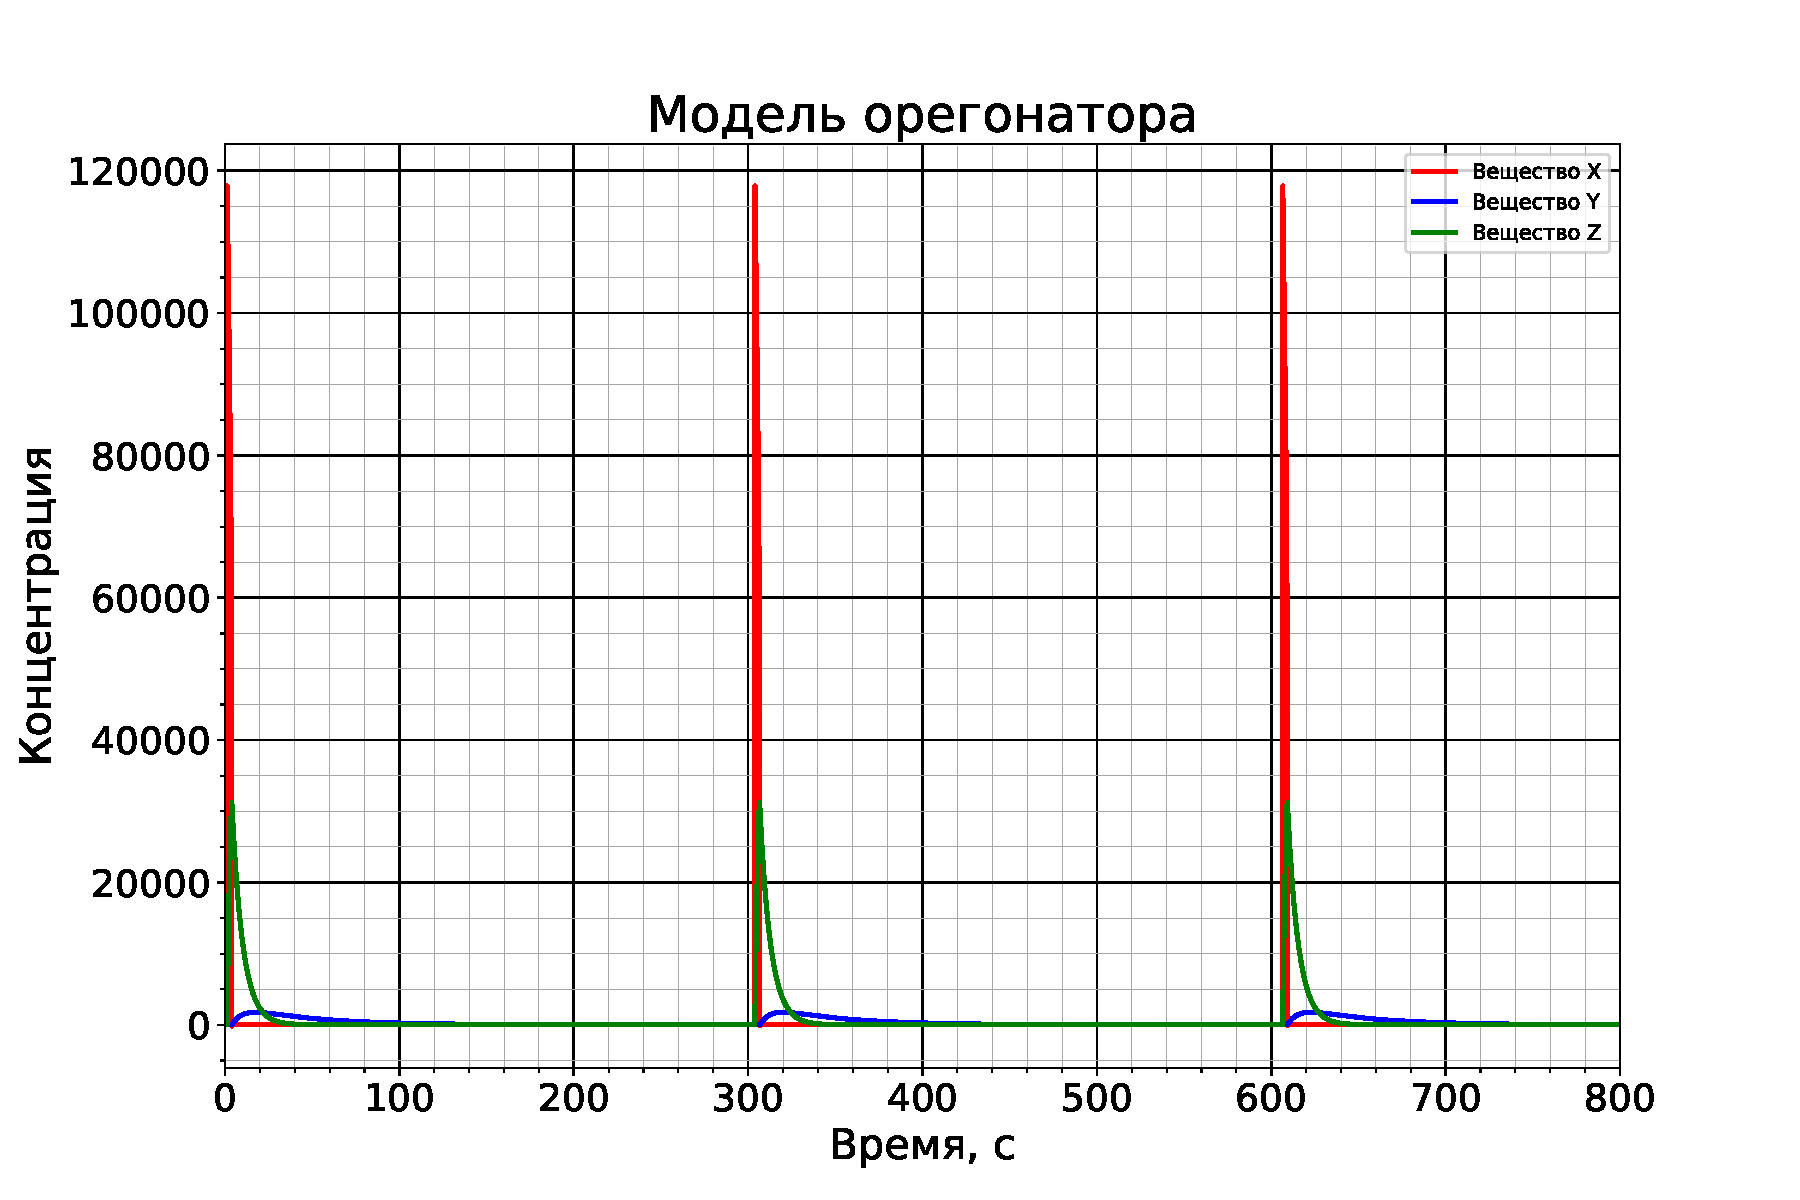
\includegraphics[width=1.1\linewidth]{Pictures/Full.pdf}
			\caption{Графики решения системы}
		\end{figure}
	
		Видно, что решение периодическое. Также виден резкий всплеск концентрации вещества X. Если посмотреть на главную часть поближе, то увидим следующее:
		\begin{figure}[h!]
			\centering
			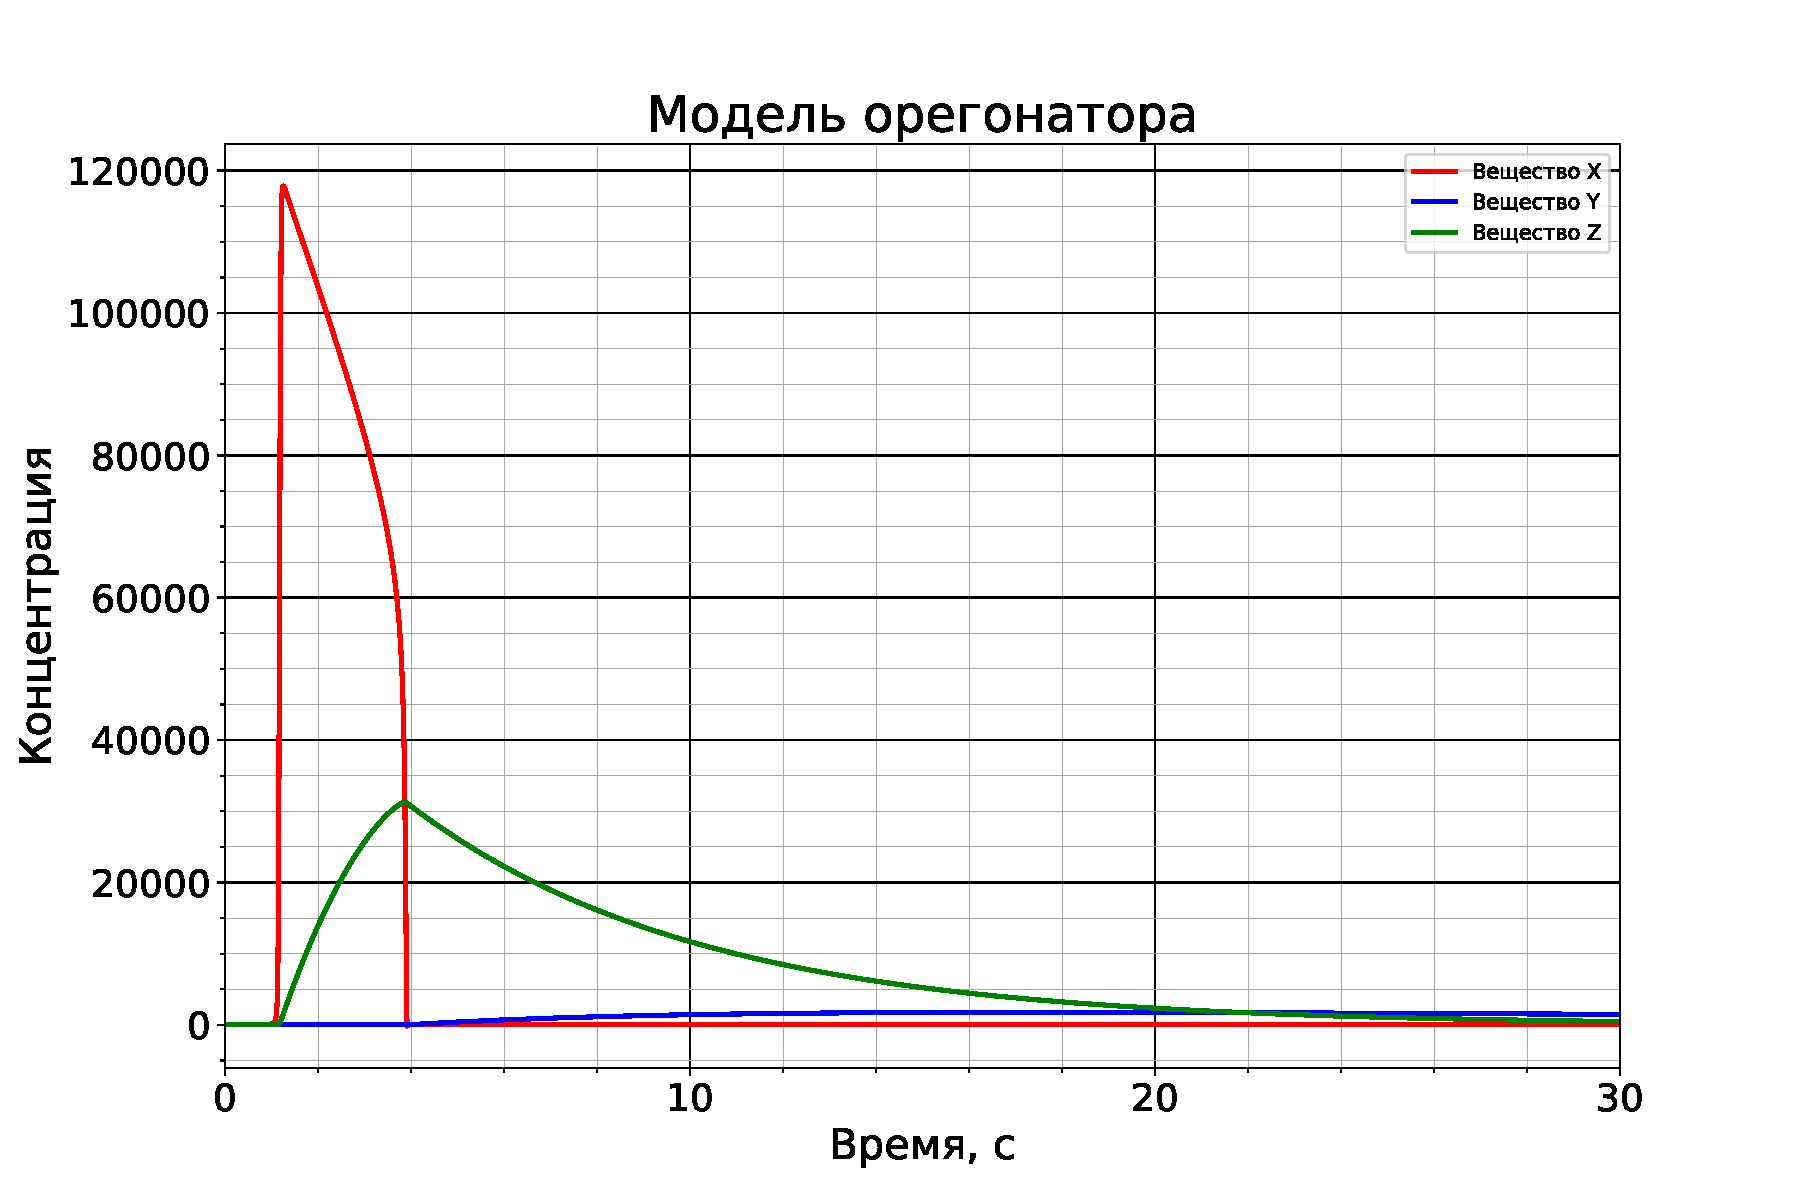
\includegraphics[width=1.1\linewidth]{Pictures/Part.pdf}
			\caption{Главная интересующая часть решения}
		\end{figure}
	
		То есть быстротекущий процесс связан с веществом X, а медленные -- с Y и Z.
		
		Также, можем взглянуть на отдельный пик поближе:
		\newpage
		\begin{figure}[h!]
			\centering
			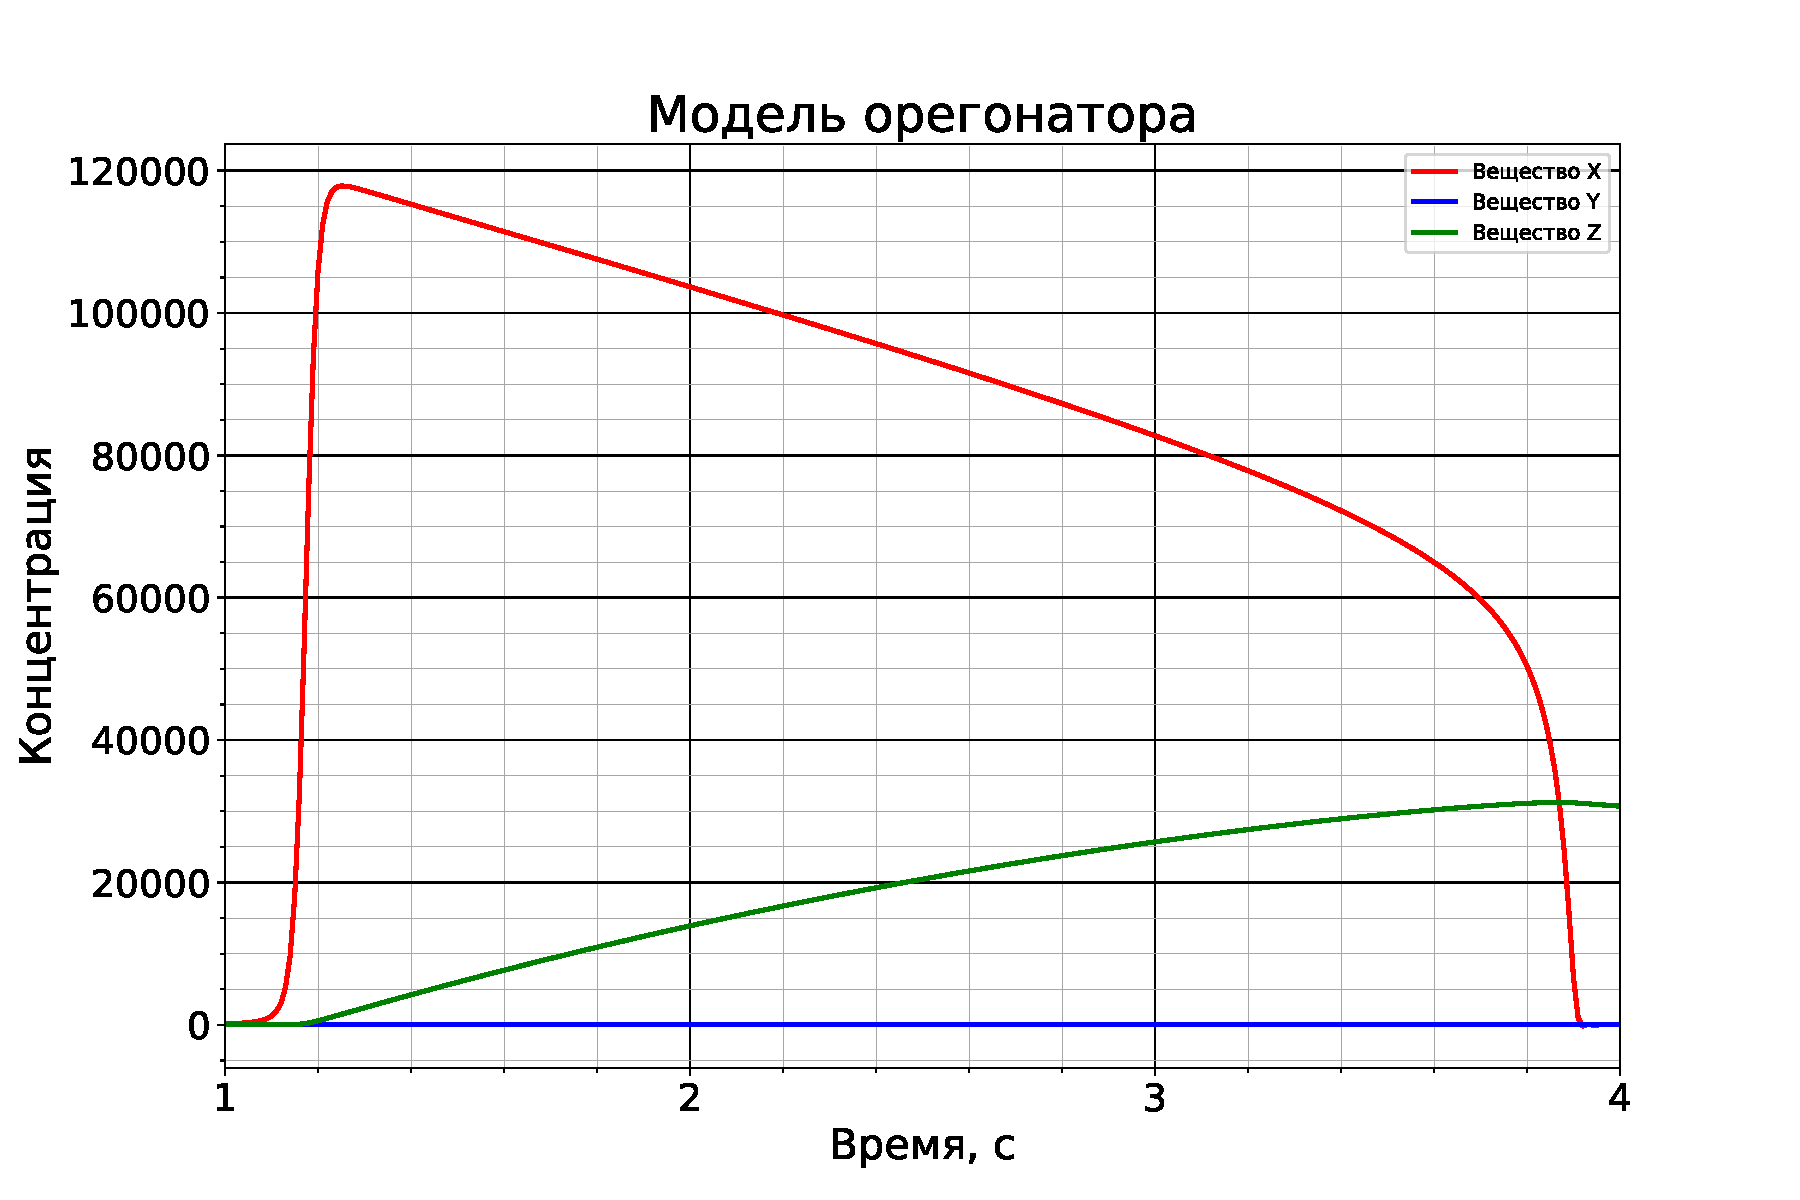
\includegraphics[width=1.1\linewidth]{Pictures/OnePeak.pdf}
			\caption{Вид резкого всплеска концентрации вещества X}
		\end{figure}
		
		\tocsection{Вывод}
		В работе был реализован один из методов решения жестких систем обыкновенных дифференциальных уравнений, а именно -- трехстадийный метод Розенброка. С помощью него была решена система, которая является жесткой. Процесс небыстрый, однако с его помощью можно хоть как-то решать жесткие системы.
		
		
\end{document}